\startfirstchapter{Introduction}
\label{chapter:introduction}

Start with 2-3 introductory paragraphs which present the search and summarize the results, as well as how they fit into the wider search for dark matter. 

\section{Introduction to the Standard Model}

The Standard Model (SM) describes all known elementary particles and three of the four known forces by which they interact with one another - the strong, the electromagnetic, and weak forces. The theory of general relativity, which describes the gravitational force, has yet to be incorporated into the SM. 

The known particles, illustrated in Figure \ref{fig:standard_model} are divided into two classes known as ``fermions" and ``bosons" on the basis of an intrinsic form of angular momentum known as ``spin". Fermions carry spin \(\frac{1}{2}\) and bosons carry integer spin. 

The specific forces by which particles in the SM interact with one another are determined by the charge(s) that they carry. Particles carrying electric charge interact with other particles carrying this charge via the electromagnetic force. Similarly, particles carrying weak and colour charge interact via the weak and strong forces, respectively. 

Each fermion has a corresponding anti-particle with the same mass, but with opposite values of the charges carried - for example, the electron carries negative electric charge and its antiparticle, the positron, carries positive electric charge. 

\begin{figure}[H]
	\centering
	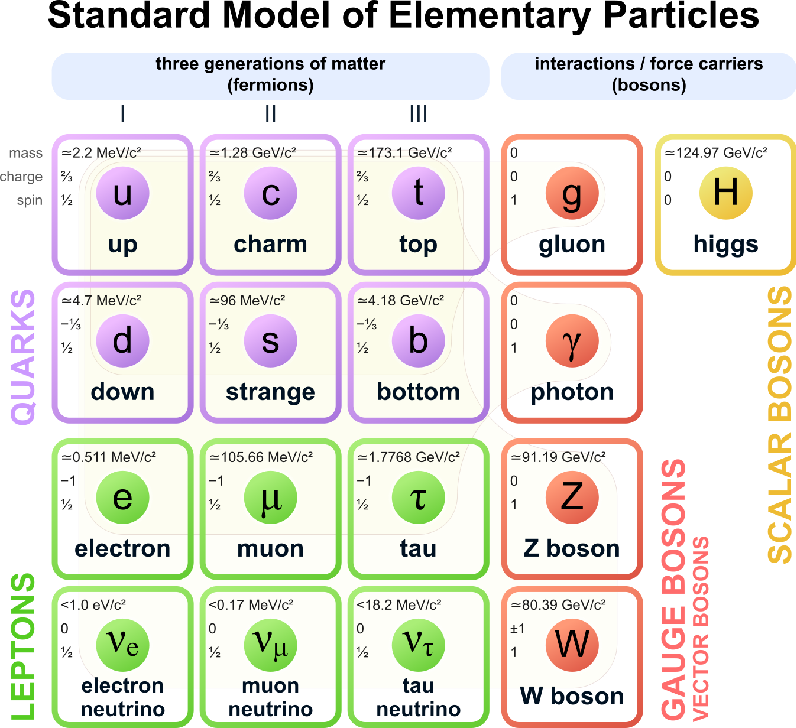
\includegraphics[width=0.7\textwidth]{Figures/1/StandardModel.pdf}
	\caption[]{Names and fundamental properties of particles in the Standard Model}
	\label{fig:standard_model}
\end{figure}

\subsection{Fermions}

Fermions are further sub-divided into leptons and quarks, depending on the charges they carry, and hence the forces by which they interact. There are three known generations of fermions, labelled I, II and III in Figure \ref{fig:standard_model}, each with significantly higher mass than the last. Each generation contains a pair of quarks and a pair of leptons, along with their associated antiparticles. The quark pair consists of one ``up-type" quark with positive electric charge and one ``down-type" with negative charge. The lepton pair consists of one charged lepton and one charge-neutral ``neutrino". 

Leptons carry electric charge and weak isospin, and as a result interact with one another and with other particles carrying these charges via the electromagnetic and weak forces, respectively.  

Quarks also carry electric charge and weak isospin, and additionally carry colour charge. The colour charge allows quarks to interact via the strong force, such that quarks interact by all three forces described by the SM. Unlike charged leptons, which carry an electric charge of \(\pm1\), quarks carry fractional electric charged; up-type quarks carry a charge of \(+\frac{2}{3}\) and down-type carry a charge of \(-\frac{1}{3}\).

Due to an effect known as ``colour confinement", quarks cannot exist as stable particles in isolation, and must instead combine with other quarks to form stable ``colour-neutral" states called ``hadrons". The two major forms of hadrons are ``mesons" formed by a quark-antiquark pair and ``baryons" formed by three quarks. Due to the strength of the strong interaction, there is a relatively high probability that particle production and decay initiated by high energy $pp$ collisions at the LHC will proceed via strong force interactions compared with other forces. As a result, the vast majority of decay products observed in the ATLAS detector are cascades of hadronic interactions in the calorimeter referred to as ``jets" \footnote{See Section \ref{sec:had_calo} for a more detailed discussion of jets in the hadronic calorimeter.} which are initiated by hadrons produced in the collisons.

\subsection{Bosons}

Bosons in the SM are divided into ``gauge bosons" and ``scalar bosons". The gauge bosons are spin 1 force carriers which mediate interactions between particles. The photon mediates electromagnetic interactions between electrically charged particles. The gluon mediates the strong interaction between quarks. Unlike photons which are charge-neutral, the gluon itself carries colour charge, which allows it to self-interact via the strong force. The weak force is mediated by three particles: the electrically neutral Z boson, and two W bosons (W$^\pm$) with opposite electric charges of $\pm$1. 

Scalar bosons are defined as spin 0 particles. There is only one known scalar boson in the SM, namely the Higgs boson (or, simply, the ``Higgs"). Particles in the SM acquire mass via their interaction with the Higgs field. As such, the Higgs only interacts with massive SM particles, which includes all particles except the photon and the gluon. The more massive the particle, the greater its interaction strength - i.e. probability of interaction - with the Higgs. Neutrinos are a possible exception; there is at present no mechanism in the SM by which neutrinos could interact with the Higgs field, so the origin of their tiny masses remains an open question.  

\subsection{Mathematical Formulation of the Standard Model}

The SM is formulated mathematically as a quantum field theory, in which particles of the SM are represented as excitations of quantum fields of spacetime \(x\). The mathematical formulation of the SM is presented in detail in standard texts \cite{griffiths_2008, SM_intro}, and briefly summarized in this section, with focus placed on aspects that are relevant to later discussions in this thesis.

\subsubsection{Lagrangian Densities}

As in classical field theories, the quantum fields of the SM and their interactions are powerfully described by the formalism of Lagrangian densities, which are functions of the quantum fields and their derivatives. For example, interactions between photons and electrically charged fermions are described in quantum electrodynamics (QED) by the following Lagrangian density term:

\begin{equation}
\label{eq:qed_interaction}
\mathcal{L}_\text{QED, interaction} = -q\psi^\dagger(x)\gamma^0\gamma^\mu\psi(x) A_\mu(x)
\end{equation}

\noindent where \(\psi(x)\) represents the spinor field of the spin-\(\frac{1}{2}\) fermions in the SM, \(A_\mu(x)\) represents the vector field of the massless spin-1 photon and \(\gamma^\mu\) are the Dirac matrices \cite{griffiths_2008}. The index \(\mu\) runs over the four spacetime coordinates. The factor \(q\) represents the charge of the fermion involved in the interaction, and its value - \(\pm1\) for charged leptons, \(+\frac{2}{3}\) (\(-\frac{1}{3}\)) for up (down) type quarks and 0 for neutrinos - determines the strength of the interaction. 

\subsubsection{Symmetries and Groups Theory Description}

Symmetries in the Lagrangian densities are described in the language of group theory by classifying the fundamental interactions into gauge groups which describe their symmetries. For example, QED exhibits a symmetry under local phase transformation, described by the unitary local gauge group U(1). This means that the Lagrangian \(\mathcal{L}_\text{QED}\) is invariant under the multiplication of the fermion spinor \(\psi\) by a unitary \(1\times1\) matrix U (\(U^\dagger U=1\)), which represents a local phase transformation \(U = e^{i\theta(x)}\) where \(\theta(x)\) can be any function of the spacetime coordinates \(x\). This symmetry is ensured by the inclusion of the vector field \(A_\mu(x)\) in the QED Lagrangian, which is identified with the physical photon. Because it ensures invariance under the U(1) gauge group, the vector field \(A_\mu(x)\) is referred to as a ``gauge field", and the corresponding boson (the photon) as a ``gauge boson". The symmetries in the SM are described by the direct product\footnote{General definitions of group theory can be found, for example, in Section 1.1 of Ref. \cite{costa2012symmetries}.} of U(1)\(\times\)SU(2)\(\times\)SU(3) gauge groups. 

\subsubsection{Quantum Chromodynamics}

The theory of quantum chromodynamics (QCD) \cite{qcd_2007}, which describes the strong interactions mediated by gluons between particles with colour charge (quarks and gluons) is described by the SU(3) gauge group. The quarks are represented by a three-component vector of spinors: \(\psi_c = \{\psi_r, \psi_b, \psi_g\}\), where the subscripts refer to the three colours that constitute the charges of the strong interaction. The QCD Lagrangian (see eg. Eq. 10.88 in Ref. \cite{griffiths_2008}) is symmetric under a transformation of the quark spinor \(\psi_c\) by a \(3\times3\) SU(3) matrix which is unitary with determinant 1. The SU(3) symmetry is ensured by the presence of an eight-component set \(\boldsymbol{\boldsymbol{A}^\mu}\) of vector gauge fields in the QCD Lagrangian associated with massless gauge bosons. The massless gauge bosons are identified as the eight physical gluons, where each of the eight physical gluons possesses a unique superposition of \({rgb}\) colour states \cite{griffiths_2008}.

\subsubsection{Electoweak Theory and the Higgs Mechanism}

The mathematical descriptions of the weak and electromagnetic forces are unified into a single ``electroweak" \cite{electroweak_2012} theory whose symmetries are described by the SU(2)\(\times\)U(1) product of gauge groups. 

Yang-Mills theory \cite{yang_mills_1954} shows that a set of three vector gauge fields associated with massless gauge bosons are needed to satisfy the SU(2) symmetry, and a fourth massless vector gauge boson is needed to satisfy the U(1) symmetry. The three-component set of vector bosons required to satisfy the SU(2) symmetry are identified as the ``weak isospin triplet" \(\boldsymbol{W}\), and the single gauge boson needed to satisfy the U(1) symmetry as the singlet \(B\). 

The SU(2)\(\times\)U(1) symmetry of the SM Lagrangian does not admit mass terms of the form \(m_X^2X^\dagger X\), where X is an arbitrary field. Masses of the physical \(W^\pm\) and \(Z\) bosons, and all other massive particles in the SM are generated by the ``Higgs mechanism" \cite{HiggsTheory1,HiggsTheory2,HiggsTheory3}, which adds the following term to the SM Lagrangian:

\begin{equation}
\label{eq:higgs_lagrangian}
\mathcal{L}_\text{Higgs} = (D^\mu H)^\dagger(D_\mu H) - V(H)
\end{equation}

\noindent where \(H\) is a complex scalar field whose symmetries are described by the SU(2) group:

\begin{equation}
H = \frac{1}{\sqrt{2}}
\begin{pmatrix}
0 \\
h+v
\end{pmatrix}
\end{equation}

\noindent where \(h(x)\) is interpreted as the scalar field of the physical Higgs boson, and \(v\) is the vacuum expectation value. With \(H\) in this form, \(\mathcal{L}_\text{Higgs}\) is described by the U(1) symmetry group but not the SU(2) group, and is thus said to ``break" the electroweak symmetry SU(2)\(times\)U(1) to the QED gauge symmetry U(1).

The covariant derivative \(D_\mu H\) in Eq. \ref{eq:higgs_lagrangian} takes the form:

\begin{equation}
\label{eq:D_muH}
D_\mu H = \big(\partial_\mu + i\frac{1}{2}g\sigma_k W^k_\mu+i\frac{1}{2}g'B_\mu\big)H
\end{equation}

\noindent where \(\sigma_k\) are the Pauli matrices, and \(g\) and \(g'\) are the coupling constants between the Higgs field and the \(\boldsymbol{W}\) and \(\boldsymbol{B}\) fields, respectively.

The Higgs potential \(V(H)\) takes the form 

\begin{equation}
V(H) = -\mu^2H\dagger H + \lambda(H^\dagger H)^2
\end{equation}

\noindent where the second term describes quartic self-interactions of the Higgs field.

The emergence of the massive physical \(W^\pm\), \(Z\) bosons and the massless photon comes from the interaction between the 

 can be seen by expanding Eq. \ref{eq:D_muH}, considering only the terms involving the vacuum expectation value \(v\):

\begin{equation}
\label{eq:higgs_expanded}
\mathcal{L}_\text{Higgs} = \frac{v^2}{8}\Big[g^2\big((W^1_\mu)^2+(W_mu^2)^2\big) + (gW^3_\mu-g'B_\mu)^2\Big] + ...
\end{equation}

With the physical vector boson fields and masses defined as:

\begin{equation}
\begin{split}
W^\pm_\mu & \equiv \frac{1}{2}(W_\mu^1 \mp W_\mu^2) \phantom{xxxxxxxxxlxx}\text{ with mass }\phantom{xxx} m_W=\frac{gv}{2} \\
Z_\mu & \equiv \frac{1}{\sqrt{g^2+g'^2}}(gW_\mu^3-g'B_\mu) \phantom{xxx}\text{ with mass }\phantom{xxx} m_Z = \frac{v}{2}\sqrt{g^2+g'^2} \\
A_\mu & \equiv \frac{1}{\sqrt{g^2+g'^2}}(g'W^3_\mu+gB_\mu) \phantom{xxx}\text{ with mass }\phantom{xxx} m_A = 0
\end{split}
\end{equation}

It can be readily confirmed that Eq. \ref{eq:higgs_expanded} takes the form \(\mathcal{L}_\text{Higgs} = \big[(W^\pm)_\mu^\dagger(W^\pm)^\mu + Z_\mu^\dagger Z^\mu + A_\mu^\dagger A^\mu\big] + ...\). Masses of fermions are likewise generated by so-called Yukawa couplings \cite{weinberg_1967} between the fermion and Higgs fields. The dark Higgs model used to optimize and interpret the DM search presented in this thesis postulates that particles in the dark sector would acquire their masses by means of their interaction with the dark Higgs field \(S\), as discussed in Chapter \ref{chapter:dh_model}. 

\subsection{Particle Decay and Lifetime}

The lowest-mass ``first-generation" quarks and leptons that comprise column I in Figure \ref{fig:standard_model}, along with the massless photons and gluons, are the only stable particles in the SM. All other particles are unstable, and will decay to less-massive particles after they are produced. The decay of an unstable particle occurs randomly with respect to the time elapsed since the particle was produced. However, this random process is governed by Poisson statistics, and the likelihood that an unstable particle will remain after some period \(t\) decays exponentially, with a mean lifetime \(\tau\) in the particle's rest frame:

\begin{equation}
\label{eq:particle_decay}
P(t) = e^{\frac{t}{\tau}}
\end{equation}

\noindent where the decay rate \(\Gamma\) is the inverse of the mean lifetime.  

\subsection{Collision and Decay Processes at Colliders}
\label{sec:col_decay_procs}

The high-energy counter-rotating proton beams at the LHC are brought into head-on collisions at four interaction points around the ring, each of which is surrounded by a detector\footnote{See Chapter \ref{chapter:lhc_atlas} for a detailed discussion of the LHC and the detectors which surround the four interaction points.}. At each interaction point, constituents of the colliding protons known as ``partons"\footnote{See Section \ref{sec:parton_model} for an introduction to the parton model.} can pair annihilate to form observable collision products via one or more ``virtual mediators"\footnote{See Section \ref{sec:virtual_particles} for a discussion of virtual particles.}, and the collision products are subsequently measured by the detector. 

Each process that describes a mechanism by which partons may annihilate to form observable products has a certain probability of taking place relative to other possible annihilation and production processes. The probability that a given process will take place is quantified by its ``cross section" \(\sigma\). The beam luminosity \(\mathcal{L}\) relates the rate of collisions \(\frac{dN}{dt}\) which proceed via a given process to the cross section of the process:

\begin{equation}
\frac{dN}{dt} = \mathcal{L}\sigma
\end{equation}

The luminosity can be integrated over a period of time \(t_1\) to \(t_2\), such that the total number of events expected to be produced via a process with cross section \(\sigma\) over the given period is related to the ``integrated luminosity" \(\mathcal{L}_\text{int}\) by:

\begin{equation}
\label{eq:integrated_lumi}
N = \sigma\int_{t_1}^{t_2}\mathcal{L}(t)dt = \sigma\mathcal{L}_\text{int}
\end{equation}

\subsubsection{Feynman Diagrams}

The interaction mechanisms by which observable collision products are produced from the annihilation of two partons can be represented by Feynman diagrams, which are described in detail in Chapter 2 of Ref. \cite{griffiths_2008} and summarized here. As an example, the Feynman diagram for the Drell Yan process in which a \(q\bar{q}\) pair annihilate to form a lepton pair \(\ell\bar{ell}\) via a virtual photon \(\gamma^{*}\) or Z boson \(Z^{*}\) mediator is shown in Figure \ref{fig:drell_yan}. 

The particles involved in the interactions are represented as lines in a Feynman diagram, with different particle types represented by different line styles - fermions are generally represented by solid straight lines, and bosons (with the exception of gluons) are generally represented by wavy lines. Particle interactions are represented by vertices at which the lines in the diagram intersect. The \(q\bar{q}\) annihilation to form the virtual \(\gamma^{*}/Z^{*}\) mediator is represented in Figure \ref{fig:drell_yan} by the vertex at which the \(q\) and \(\bar{q}\) fermion lines meet the \(\gamma^{*}/Z^{*}\) boson line, and the subsequent decay of the  \(\gamma^{*}/Z^{*}\) to \(\ell\bar{\ell}\) is represented by the vertex to the right at which the \(\gamma^{*}/Z^{*}\) line meets the \(\ell\) and \(\bar{\ell}\) lines. Note that time flows horizontally from left to right in Feynman diagrams, so the colliding \(q\bar{q}\) pair are shown on the left and the observable decay products \(\ell\bar{\ell}\) on the right.

\begin{figure}[hp]
	\centering
%	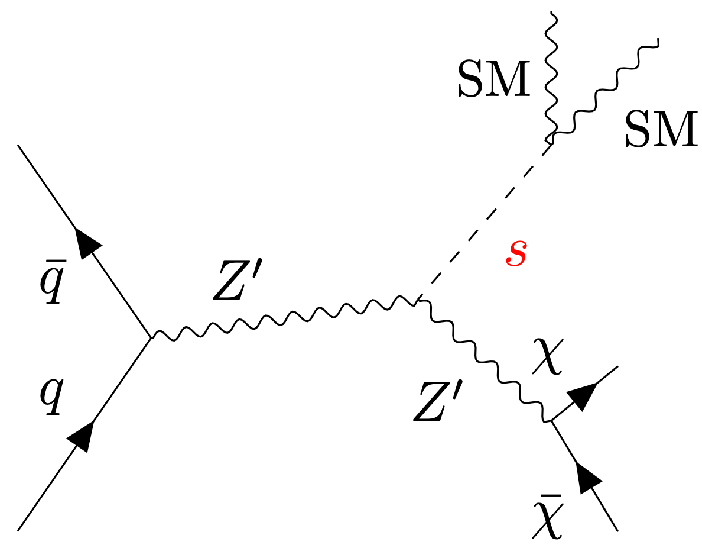
\includegraphics[width=0.95\textwidth]{Figures/2/Fey1.pdf}
		\begin{tikzpicture}
			\begin{feynman}

		 		\vertex (a1);
		 		\vertex at ($(a1) + (0cm, -3cm)$) (b1);
		 		\vertex at ($(a1) + (1cm, -1.5cm)$) (c1); %gamma/Z
		 		\vertex at ($(c1) + (2cm, 0cm)$) (c2); %gamma/Z
				\vertex at ($(c2) + (1cm, -1.5cm)$) (d1);
				\vertex at ($(c2) + (1cm, 1.5cm)$) (d2);

		 		\diagram* {
		 		  {[edges=fermion]
		 		    (b1) -- [edge label=\(q\)]( c1) -- [edge label=\(\bar{q}\)](a1),
				    (d1) -- [edge label=\(\bar{\ell}\)]( c2) -- [edge label=\(\bar{\ell}\)](d2),
		 		  },
		 		  (c1) -- [boson, edge label=\(\gamma^{*}/Z^{*}\)] (c2),
		 		};
		 	\end{feynman}
		 \end{tikzpicture}
	\caption{Feynman diagram for the Drell Yan process.}
	\label{fig:drell_yan}
\end{figure}

\subsubsection{Virtual Particles}
\label{sec:virtual_particles}

In general, ingoing and outgoing lines in a Feynman diagram represent real observable particles, and internal lines represent so-called virtual particles. Virtual particles are not observable, but are rather a representation of the mechanism involved with producing the observable final state products. Importantly, virtual particles are not in general produced with the mass of their corresponding real particle, but can in principle take on whatever mass is needed to satisfy energy and momentum conservation at each interaction vertex that they are involved with. However, the more ``off-shell" the mass of the virtual particle, meaning the more it differs from the mass of the corresponding real particle, the lower is the production cross section \(\sigma(m^{*})\) with which the process would be expected to proceed for the given mass \(m^{*}\) of the virtual particle required to satisfy energy-momentum conservation. This relationship is described quantitatively by the Breit-Wigner formula \cite{breit_wigner}:

\begin{equation}
\label{eq:breit_wigner}
\sigma(m^{*}) \propto \frac{1}{(m^{*}-m_0)^2 + \frac{\Gamma_E^2}{4}}
\end{equation}

\noindent where \(m_0\) is the ``on-shell" mass of the corresponding real particle, and \(\Gamma\) is the total decay width of the real particle. The Breit-Wigner formula describes a peak centred at \(m_0\) with width \(\Gamma_E\). The lifetime of the corresponding particle is related to the width of its Breit-Wigner resonance by \(\tau = \frac{\hbar}{\Gamma_E}\).

\subsubsection{Matrix Element}

%In order to study collision events measured by particle detectors at the LHC, it is important to calculate the rate at which the detector would be expected to measure collision events which proceed by different processes, such as the Drell-Yan process shown in Figure \ref{fig:drell_yan}. 

The cross section associated with a process of particle production from \(pp\) collisions at the LHC, such as the Drell-Yan process shown in Figure \ref{fig:drell_yan}, is in general proportional to an integral of the squared matrix element \(|\mathcal{M(\boldsymbol{x}, \boldsymbol{\alpha})}|^2\):

\begin{equation}
\label{eq:matrix_element}
\sigma \propto \int|\mathcal{M(\boldsymbol{x}, \boldsymbol{\alpha})}|^2 d\boldsymbol{x} 
\end{equation}

\noindent where the quantities \(\boldsymbol{x}\) describe the dynamics (masses, momenta, quantum numbers, etc.) of the incoming and outgoing observable particles, and \(\boldsymbol{\alpha}\) are terms which describe the internal structure process represented by the Feynman diagram, including the coupling constants which quantify the interaction strength of the particles involved at each interaction vertex and an integration over the possible dynamics of the virtual particles. 


\section{Evidence for Dark Matter from Observational Astronomy}

Many independent lines of astronomical observation collectively provide compelling evidence for the presence and abundance of a form of matter in the universe that is distinct from the matter that constitutes stars and planets, and which is not directly observable because it neither emits nor absorbs light. Some of the earliest and clearest evidence for this so-called ``dark matter" came in 1978, when Rubin et al. \cite{Rubin_et_al} reported systematic anomalies in their observations of the rotation speeds of spiral galaxies. In particular, it was found that distributions of the rotation speed as a function of the radial distance from the galactic centre differed in shape from what would be naively expected on the basis of the distribution of galactic mass measured from the observed luminosity profile. 

\begin{figure}[H]
	\centering
	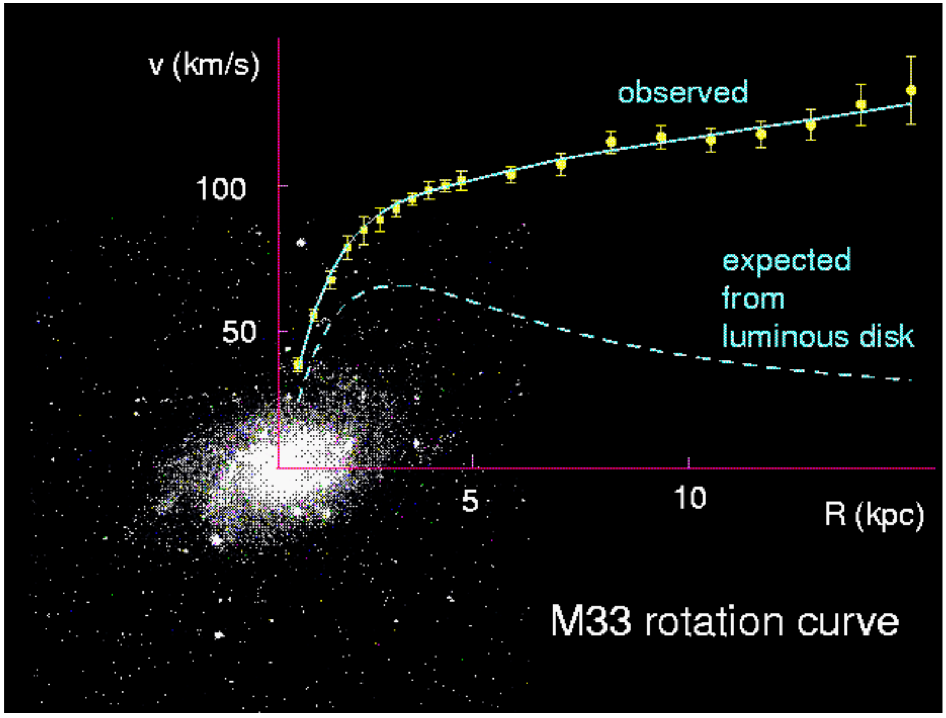
\includegraphics[width=0.7\textwidth]{Figures/1/m33_rotation.pdf}
	\caption[]{Observed rotation speed of the nearby dwarf galaxy M33, overlaid on an optical image of the galaxy. Yellow data points show observed rotational speed of the galaxy as a function of the radial distance from the galactic centre (in kpc). Dashed line shows the expected rotational speed on the basis of the calculated mass of the luminous stellar disk. }
	\label{fig:m33_rotation}
\end{figure}

At the time, spiral galaxies had been observed to be comprised of a central spheroidal ``galaxy bulge" which contains the majority of luminous matter in the galaxy, in addition to a ``disk" extending out to larger radii, for which the luminous matter falls off exponentially. Assuming that the distribution of mass in the spiral galaxy follows the luminosity profile, application of Newtonian gravitational mechanics would predict the rotation speed to peak near the edge of the central galaxy bulge, as illustrated in the blue dashed line in Figure \ref{fig:m33_rotation} for the dwarf galaxy M33, and fall off beyond due to the exponentially decaying matter density of the disk. However, the observed galactic rotation speed, shown with yellow data points in Figure \ref{fig:m33_rotation}, is generally observed to continue increasing well beyond the luminous galactic bulge. These anomalies in galactic rotation curves, which have since been observed in hundreds of spiral galaxies \cite{rotn_curves_1995}, can be explained by postulating an additional source of non-luminous matter density in galaxies, known today as ``dark matter", would extend well beyond the luminous bulge, provide the necessary gravitational potential to prevent the rotation speeds from falling off beyond the bulge.

In the years following these early reports of anomalous galactic rotation curves which suggested the existence of dark matter in galaxies, modifications to the laws of Newtonian gravity at galactic scales \cite{mond_1983} were also considered as an alternative to dark matter to explain the observed anomalies. However, while the proposed modifications to gravity were successful in describing the observed galactic rotation curves, numerous lines of astronomical observations in other contexts have independently turned up discrepancies between the observed content of total and luminous matter which would either require further modifications to the laws of gravity, or simply cannot be readily explained by modifying the laws of gravity, thus lending strong confidence hypothesis that a large fraction of the matter density of the universe is non-luminous. Additional evidence at galactic scales comes from strong differences between the spatial distributions of matter density, measured using gravitational lensing, and of luminous matter following collisions of galaxy clusters \cite{bullet_1995}, indicating that the majority of the matter density in the colliding galaxies is non-luminous. Studies of the relative contribution to the masses of galaxy clusters from luminous matter using data from the Chandra X-ray observatory \cite{Chandra_2013} suggest that only 15-20\% of the mass composition of the galaxies studied was comprised of luminous matter.

Because of their stability and electromagnetic interactions, protons and neutrons comprised of bound quarks, as well as their bound electrons - collectively known as ``baryonic matter" - comprise by mass the overwhelming majority of known luminous matter in the universe. Precision measurements of the abundance of light nuclei - D, 3He, \(^4\)He, and \(^7\)Li  produced in the early universe following the big bang - known as big bang nucleosynthesis \cite{pdg_2018} - indicate that baryonic matter constitutes approximately 5\% \cite{pdg_2018} of the energy density of the universe. Current measurements of anisotropies in the cosmic microwave background \cite{cmb_1965} measured by the Planck collaboration \cite{Planck_2020} interpreted in the context of the standard \(\Lambda\)CDM model of cosmology \cite{pdg_2018} indicate that approximately 30\% of the energy density of the universe is comprised of matter, with the missing 25\% identified as non-baryonic dark matter. This result implies that \(~85\%\) of all matter in the universe is comprised of non-luminous dark matter, consistent with the findings discussed above from measurements of galaxy clusters.

\section{Dark Matter Composition Hypotheses}

There is at this stage a diverse of astronomical observations which consistently point to the need for a non-luminous form of non-baryonic matter known as dark matter, in the universe. While active research continues within the theoretical community \cite{mond_2012, mond_2021} into the possibility of modifying the laws of gravitation at astronomical scales to explain these observations without the need for dark matter, there are significant theoretical challenges involved with designing modifications that can consistently explain the range of observational anomalies at scales ranging from individual galaxies to galaxy clusters, while simultaneously addressing the apparent need for dark matter at cosmological scales from the discrepancy between measurements of the baryonic mass density from BBN and the much larger total mass density inferred from anisotropies in the CMB. As a result, dark matter is widely considered most theoretically well motivated hypothesis to explain the full range of observational data.

While the astronomical observations provide a wealth of information regarding the composition of dark matter in the universe by means of its gravitational effects on visible matter, they provide relatively few clues as to what actually comprises the dark matter. Its abundance in the present day universe indicates that it must be stable on cosmological timescales (i.e. billions of years). The evidence from BBN and CMB anisotropies indicates that the dark matter must be non-baryonic. Its non-luminous nature further implies that it neither emits nor absorbs photons, and therefore has negligible or no charge under the electromagnetic force. Besides baryons, neutrinos represent the only other massive stable particles currently known to the SM. While the masses of individual neutrinos is relatively tiny\footnote{Current constraints from cosmology place an upper limit on the sum of neutrino masses from all generations of 0.17 eV, \(~3\times10^6\) times smaller than the electron mass}, they satisfy the requirement of being electrically neutral, which naturally leads to the question of whether there could be a sufficiently large density of neutrinos in the universe to constitute the observed dark matter density. This possibility was ruled out in the 1980's by studies \cite{neutrino_dm} which showed that the large scale structure of the universe would differ significantly from what is observed today if the mass density of the universe were dominated by neutrinos. With the stable particles of the SM ruled out, the current most widely accepted hypothesis is that dark matter is comprised of a new form of non-baryonic matter that is not currently described by the SM, and which has not yet been observed in particle detectors. 

Despite the observable effects of its gravitational interactions at astronomical scales, the strength of gravitational coupling between massive particles is \(\sim30\) orders of magnitude weaker than any of the other three forces of the SM \cite{griffiths_2008}. As a result, gravitational interactions between dark matter and SM particles are far too weak to be observable in particle detectors. Given that there have not yet been any conclusive detections of dark matter in particle detectors, 

%The fact that dark matter has not yet been observed in particle detectors leads to the questions of whether it interacts 

\begin{itemize}
\item Describe what would be gained from an experimental detection/measurement of DM
\begin{itemize}
\item Solidify the case for particle DM.
\item Measure the particle properties of DM which can't be inferred from astronomical observations - mass, interaction mechanisms with SM particles, potential interactions with other BSM particles.
\end{itemize}
\end{itemize}

\section{Dark Matter Search Strategies}
\begin{itemize}
\item Briefly introduce direct and indirect detection approaches and their relative merits
\item More detailed intro to the collider search approach and how it complements the other search modes
\begin{itemize}
\item Sharp lower bound on accessible DM masses suffered by direct detection searches due detector noise threshold is not an issue for collider searches. Neither is the neutrino floor.
\item Possibility to tailor searches to specific hypothetical DM production models by tuning selections $\rightarrow$ emphasize this point, since it's important for this search.
\item If evidence for DM found by any method (collider or otherwise), colliders can offer a superior means of pursuing dedicated measurements of its properties compared with other search modes.
\end{itemize}
\end{itemize}

\subsection{Searching for Dark Matter at Particle Accelerators}

\begin{itemize}
\item Give an idea of the breadth of accelerator DM search program.
\begin{itemize}
\item Resonance searches
\item mono-X searches
\item Model-independent and model-dependent approaches $\rightarrow$ briefly present range of model completeness, from EFT through simplified to complete.
\item Cover searches at hadron and $e^+e^-$ colliders and fixed target experiments.
\end{itemize}
\item Discuss the relative merits of searching for simplified models (bridge gap between EFT and complete theories, avoid overtuning problems inherent with complete models, facilitate adequate coverage of plausible DM production processes).
\item Briefly introduce the Dark Higgs model, and clearly identify it as a simplified model (details to be fleshed out in Chapter 2) $\rightarrow$ emphasize that this search is sensitive to heavy DM ($\gtrsim$60 GeV), with the requirement that $m_\chi>\frac{1}{2}\ms$ (to prevent the $s\rightarrow\chi\chi$ decay mode).
\end{itemize}

